\chapter{Language Model Fine-Tuning}\label{chp: Fine tuning}
\section{Adapter-Based Fine Tuning}
\paragraph{Adapters:} Adapter-based fine tuning allows for the efficient transfer of a model to multiple tasks or languages by adding small, task-specific modules called adapters to a fixed, pre-trained model. Adapters are typically small neural networks inserted between the layers of a pre-trained model as shown in Figure \ref{fig: adapter}. Each adapter only learns task-specific or language-specific features, leaving the original model weights untouched. This method is particularly advantageous for multilingual models because it enables the customization of a single foundational model for a variety of languages and tasks without the need for extensive retraining. The concept of adapter-based tuning was popularized by \citet{houlsby2019parameter}, who introduced a simple yet effective architecture for adapters as shown in Figure \ref{fig: adapter}.

\begin{figure}[hbt]
	\centering
	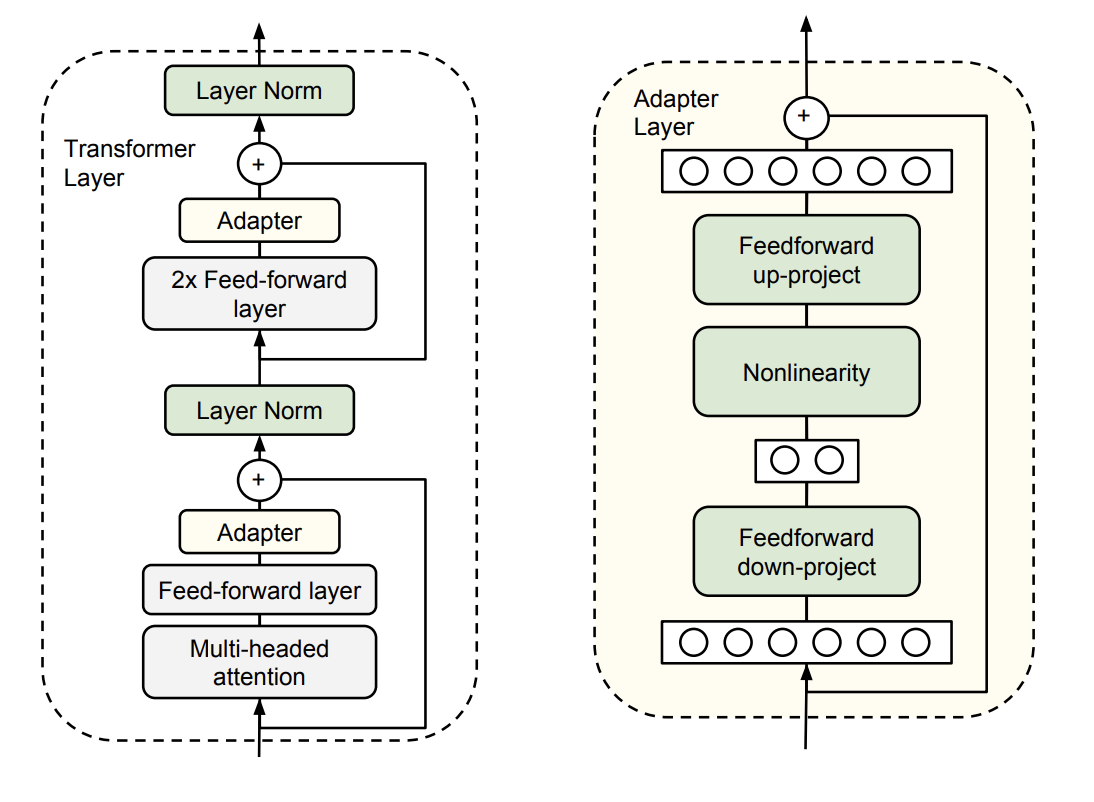
\includegraphics[width=0.75\textwidth]{adapter}
	\caption[Adapter Module Integration in the Transformer Architecture]{Adapter Module Integration in the Transformer Architecture: On the left, adapter modules are incorporated into each Transformer layer twice: once following the multi-headed attention and once after the feed-forward layers. On the right, each adapter features a bottleneck design with relatively few parameters compared to the main attention and feed-forward components of the Transformer. Each adapter includes a skip-connection for efficient training. During the process of adapter tuning, only the components shown in green, which include the adapters, layer normalization parameters, and the final classification layer (not depicted), are updated based on the downstream task data.(\citet{houlsby2019parameter})}
	\label{fig: adapter}
\end{figure}

\paragraph{MAD-X for Cross-Lingual Transfer:} Adapters have proven especially useful in multilingual settings, such as in the work by \citet{pfeiffer2020mad}, who extended the adapter approach to cross-lingual models with their MAD-X framework. MAD-X enables efficient transfer learning across languages by leveraging language-specific adapters, which capture unique linguistic characteristics of each language while sharing a common, language-agnostic model backbone.MAD-X (Multiple ADapters for Cross-lingual transfer) represents a significant evolution in the field of cross-lingual transfer, specifically designed to enhance the capabilities of pre-trained multilingual models like mBERT and XLM-R. This framework introduces a modular approach using small, additional parameter-efficient adapters to improve the model's ability to handle multiple languages and tasks efficiently.

\paragraph{Language Adapters:} Language adapters as shown in Figure \ref{fig: lang-task-adapter} are designed to adapt the model to the specificities of a given language. These adapters are trained using Masked Language Modeling (MLM) on unlabelled data from the target language. The language adapter at each layer $l$ of the transformer can be mathematically described by the following equation:
\begin{equation}
	\text{LA}_l(h_l, r_l) = U_l(\text{ReLU}(D_l(h_l))) + r_l
\end{equation}

where:
\begin{itemize}
	\item $h_l$ is the output from the previous layer or the initial input.
	\item $r_l$ is the residual connection from the previous transformer block.
	\item $D_l$ and $U_l$ are the down-projection and up-projection matrices respectively at layer $l$.
	\item $\text{ReLU}$ is the non-linear activation function.
\end{itemize}

\paragraph{Task Adapters:} Task adapters as shown in Figure \ref{fig: lang-task-adapter}, on the other hand, are used to fine-tune the model for a specific task. They are applied after the language adapters and can be described by the following equation for each layer $l$:
\begin{equation}
\text{TA}_l(h_l, r_l) = U_l(\text{ReLU}(D_l(\text{LA}_l(h_l, r_l)))) + r_l
\end{equation}

where:
\begin{itemize}
	\item $\text{LA}_l(h_l, r_l)$ is the output from the language adapter.
	\item The rest of the parameters function similarly to those in the language adapters.
\end{itemize}

\begin{figure}[hbt]
	\centering
	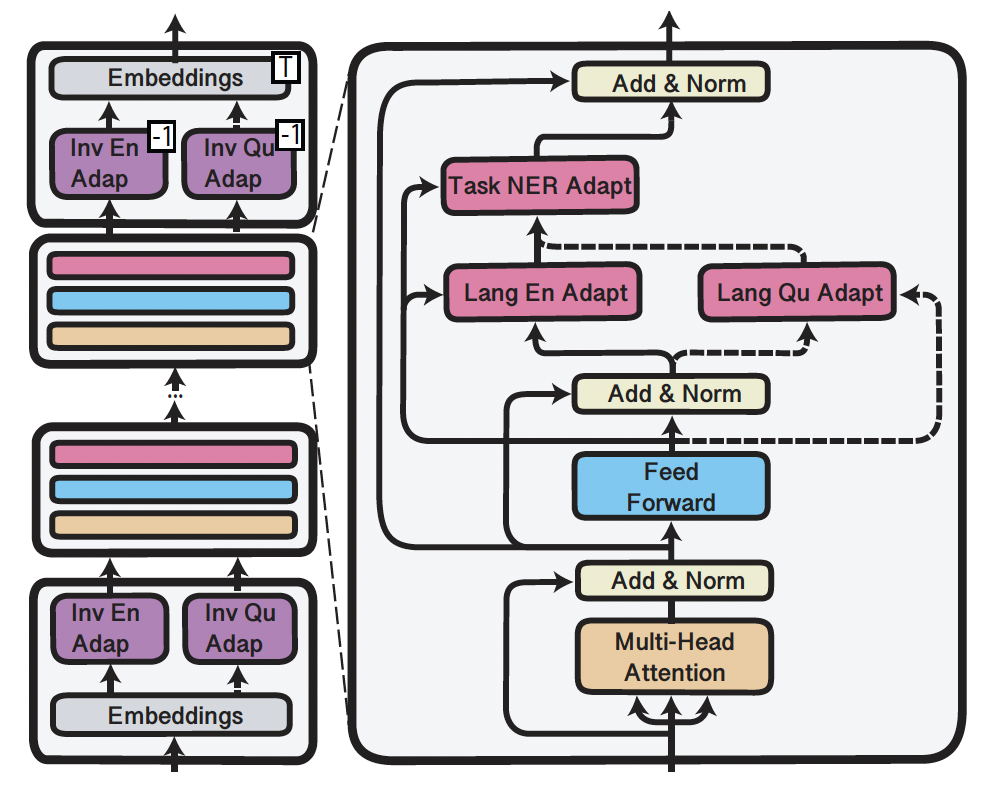
\includegraphics[width=0.75\textwidth]{lang-task-adapter}
	\caption[Overview of the MAD-X Framework in a Transformer Model]{Overview of the MAD-X Framework in a Transformer Model: Input data first passes through an invertible adapter, the output of which feeds into the model's output layer. Within each Transformer layer, language and task-specific adapters are incorporated. The language adapters, along with the invertible adapter, are trained using masked language modeling (MLM) while keeping the core multilingual model unchanged. For tasks like Named Entity Recognition (NER), task-specific adapters are added on top of the language adapters for training (illustrated with solid lines). For zero-shot cross-lingual transfer, adapters for the source language are swapped with those for the target language (shown with dashed lines).(\citet{pfeiffer2020mad})}
	\label{fig: lang-task-adapter}
\end{figure}

\paragraph{Applications:} Results by \citet{pfeiffer2020mad} demonstrate that MAD-X significantly outperforms existing state-of-the-art methods in cross-lingual transfer tasks. MAD-X delivers robust results not only in high-resource languages but also shows effectiveness in low-resource and unseen language scenarios. 

\paragraph{Limitations:} Despite its advantages, MAD-X faces several challenges:
\begin{itemize}
	\item \textbf{Model Capacity:} Pre-trained models may lack sufficient capacity to adequately represent all languages, especially those not included in the training data, leading to poorer performance in such languages.
	\item \textbf{Dependency on Source Language Quality:} The success of transfer learning heavily relies on the quality and comprehensiveness of the source language models, which can vary significantly.
\end{itemize}

\section{Generalizable Fine Tuning}
\paragraph{Child-Tuning:} Child-Tuning proposed by \citet{xu2021raise} is fine-tuning technique designed to adapt large pretrained language models (PLMs) to specific tasks by updating only a subset of the model's parameters. This approach helps to prevent overfitting and improves generalization, especially when training data is limited. Child-Tuning updates a selectively identified subset of parameters, referred to as the \emph{child network}, while keeping the rest of the model's parameters (the \emph{non-child network}) fixed. This selective updating is achieved by applying a mask to the gradients during the backward pass, effectively zeroing out the gradients for the non-child network. The standard update rule in gradient descent is given by:
\begin{equation}
	w_{t+1} = w_t - \eta \frac{\partial L}{\partial w_t}
\end{equation}

where $w_t$ represents the model parameters at iteration $t$, $\eta$ is the learning rate, and $\frac{\partial L}{\partial w_t}$ is the gradient of the loss function with respect to the parameters. In Child-Tuning, the update rule is modified to only apply to the child network, which is defined by a binary mask $M_t$. This mask is applied to the gradients, allowing only a subset of parameters to be updated:
\begin{equation}
	w_{t+1} = w_t - \eta (\frac{\partial L}{\partial w_t} \odot M_t)
\end{equation}

Here, $\odot$ denotes element-wise multiplication. The mask $M_t$ has entries of 1 for parameters belonging to the child network and 0 for others.

\paragraph{Detection of the Child Network:} The child network can be detected in two ways:
\begin{itemize}
	\item \textbf{Task-Free}: Parameters are selected based on a predefined distribution, often without specific task data. This can be seen as adding a form of regularization to prevent overfitting.
	\item \textbf{Task-Driven}: Parameters are selected based on their relevance to the specific task, typically identified through methods like Fisher Information, which measures how much information a parameter carries about the output.
\end{itemize}

\paragraph{Types of Child Tuning:} The Child-Tuning methodology introduces two variants: Child-Tuning-F and Child-Tuning-D. The former operates independently of specific task data, using a Bernoulli distribution to randomly select the child network, thereby introducing stochasticity that acts as a form of regularization. This variant aims to improve generalization by preventing overfitting to smaller datasets. On the other hand, Child-Tuning-D utilizes task-related data to identify the parameters most crucial for the task, freezing the remainder of the model to its pre-trained state. This approach not only tailors the model more closely to the task requirements but also preserves the generalization capabilities inherent in the original pre-trained model.

\paragraph{Advantages:} Child-Tuning offers several significant benefits:
\begin{itemize}
	\item \textbf{Prevention of Overfitting:} By updating only a subset of parameters, Child-Tuning prevents the model from overly adapting to the training data, thus maintaining robustness and preventing overfitting. This method has shown to improve the model's ability to generalize to new, unseen tasks and domains, improving its performance across a variety of downstream applications .
	\item \textbf{Efficient Utilization of Model Capacity:} Child-Tuning makes efficient use of a model's capacity by focusing updates on parameters that are most influential for the task at hand, therefore reducing the computational resources required for training.
\end{itemize}

\paragraph{Limitations}
Despite its advantages, Child-Tuning also encounters certain challenges:
\begin{itemize}
	\item \textbf{Dependence on Accurate Parameter Selection:} The success of Child-Tuning heavily relies on accurately identifying which parameters to include in the child network. Incorrect selections can lead to suboptimal performance.
	\item \textbf{Reduced Adaptability:} Since only a subset of parameters is updated, there might be scenarios where the non-updated parameters limit the model’s adaptability to tasks significantly different from those seen during training.
\end{itemize}

\section{Composable Sparse Fine Tuning}
\paragraph{Composable Language and Task Vectors:} Composable Sparse Fine-Tuning (CSFT) by \citet{ansell2023composable} enhances the adaptability of multilingual models by integrating task-specific and language-specific adaptations through the use of composable vectors. This method enables models to efficiently handle multiple languages and tasks without requiring separate models for each combination. CSFT operates by defining separate vectors for language and task adaptations, which are then combined to adjust the base model parameters for specific cross-lingual and task-oriented performance. The language vector, \(\phi_{\text{lang}}\), and the task vector, \(\phi_{\text{task}}\), are defined as the changes required to adapt the base model parameters \(\theta^{(0)}\) for a specific language and task, respectively:
\begin{equation}
	\phi_{\text{lang}} = \theta_{\text{lang}} - \theta^{(0)}
\end{equation}

\begin{equation}
	\phi_{\text{task}} = \theta_{\text{task}} - \theta^{(0)}
\end{equation}

where \(\theta_{\text{lang}}\) and \(\theta_{\text{task}}\) are the parameters of the model fine-tuned for the specific language and task. To achieve simultaneous adaptation to both language and task, the vectors are combined through element-wise addition:
\begin{equation}
	\phi_{\text{combined}} = \phi_{\text{lang}} + \phi_{\text{task}}
\end{equation}

This combined adaptation vector is then used to update the base model parameters:
\begin{equation}
	\theta_{\text{final}} = \theta^{(0)} + \phi_{\text{combined}}
\end{equation}

The final model, represented as \( F(\cdot; \theta_{\text{final}}) \), is thus equipped to perform the specific task in the specific language, utilizing the enhancements from both the language and task vectors as shown in Figure \ref{fig: composable-sft}.
\begin{figure}[tbh]
	\centering
	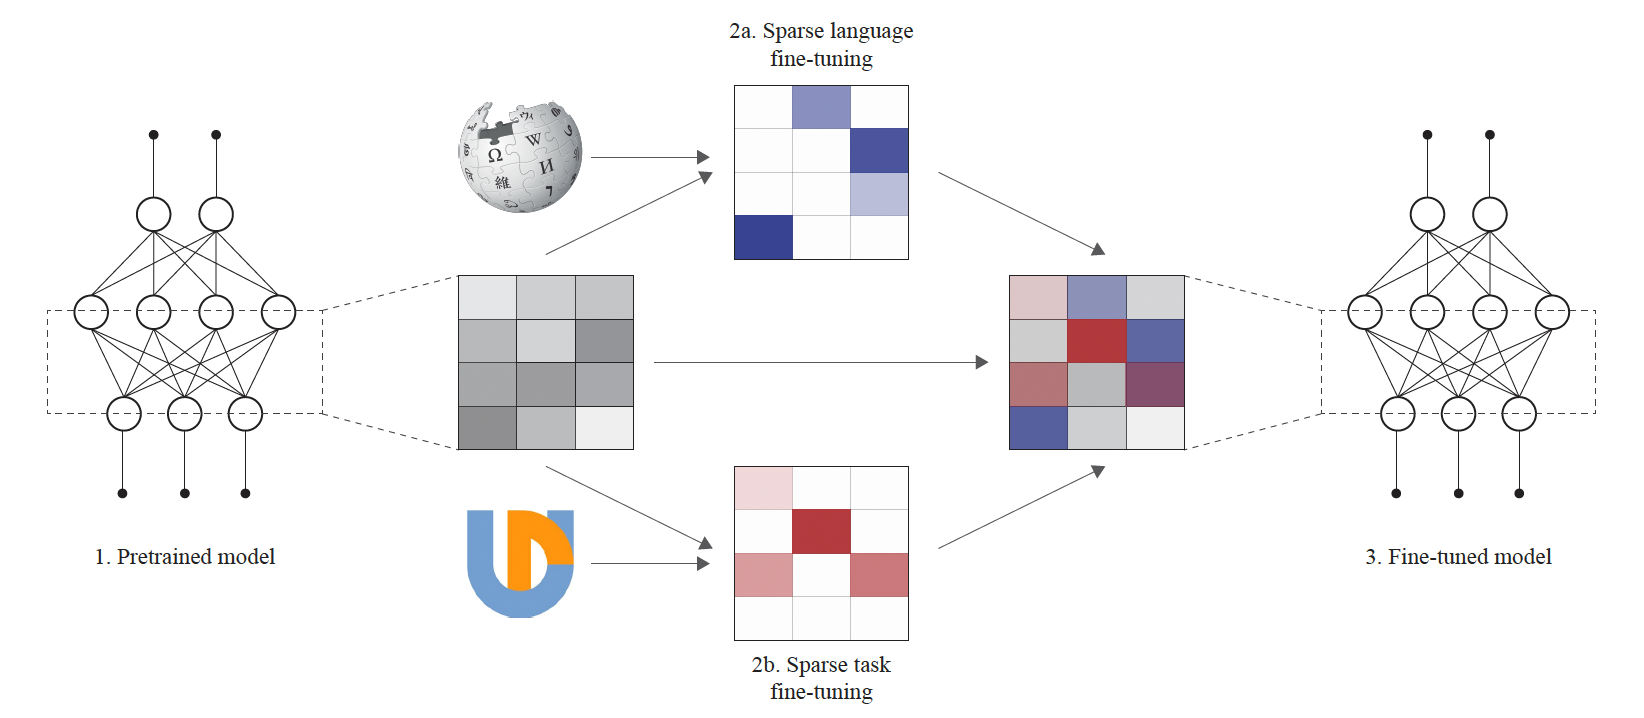
\includegraphics[width=\textwidth]{composable-sft}
	\caption[Illustration of Composable Sparse Fine-Tuning Process]{Illustration of Composable Sparse Fine-Tuning Process: Starting with the parameters of a pre-trained model shown in gray (left), we introduce task-specific and language-specific sparse fine-tunings, depicted in blue and red respectively (center). These components are then combined through addition (right) to produce the final adapted model. (\citet{ansell2023composable})}
	\label{fig: composable-sft}
\end{figure}

\paragraph{Lottery Ticket Hypothesis:} Composable Sparse Fine-Tuning (CSFT) technique is inspired by the Lottery Ticket Hypothesis by \citet{frankle2019lottery}. The Lottery Ticket Hypothesis states that within a dense neural network, there exists a smaller, sparse subnetwork (referred to as a "winning ticket") that, when trained in isolation from the beginning, can achieve comparable or even superior performance to the original, larger network. This hypothesis suggests that by identifying and training these efficient subnetworks, one can significantly reduce the computational resources required without sacrificing performance. Lottery Ticket Sparse Fine-Tuning (LT-SFT) introduces a technique inspired by the Lottery Ticket Hypothesis (LTH), specifically for multilingual models.

\paragraph{Fine Tuning Process:} The core idea behind LT-SFT is to select a subset of parameters that exhibit significant changes during initial training and fine-tune only these parameters in subsequent phases as per the LTH. LT-SFT involves two main phases:
\begin{enumerate}
	\item \textbf{Parameter Selection:} Initially, the full model parameters $\theta^{(0)}$ are trained on target data, resulting in updated parameters $\theta^{(1)}$. Parameters are then ranked based on the absolute change in their values, and a binary mask $\mu$ is constructed to identify the top $K$ parameters, where $\mu_i = 1$ if the $i$-th parameter is selected and $0$ otherwise.
	
	\item \textbf{Sparse Fine-Tuning:} Parameters are reset to their original values $\theta^{(0)}$ and only those marked by $\mu$ are updated in the subsequent training. This selective training uses the masked gradient $\mu \odot \nabla_{\theta} L(F(\cdot;\theta), D)$, where $\odot$ denotes element-wise multiplication and $L$ is the loss function.
\end{enumerate}

The sparse fine-tuning can be mathematically represented as:
\begin{equation}
	\phi = \theta^{(2)} - \theta^{(0)}
\end{equation}

where $\theta^{(2)}$ are the parameters after sparse fine-tuning. The adaptation for a task can then be expressed as a function of the base model:
\begin{equation}
	F(\cdot; \theta + \phi)
\end{equation}

This formulation allows the original model to adapt effectively to new tasks and languages by updating only a crucial subset of parameters, thereby maintaining overall model efficiency and preventing overfitting.

\paragraph{Applications:} CSFT integrates the modularity of adapters with the expressivity of sparse fine-tuning, allowing for fine-grained control over which parts of the model are updated during training. One of the key advantage of CSFT is the ability to compose these sparse tunings, which enables the application of multiple, distinct adaptations to a single model without the overhead of additional parameters at inference time. For instance, a model can be fine-tuned with a language-specific sparse tuning followed by a task-specific sparse tuning, effectively adapting the model for a specific task in a new language. The effectiveness of CSFT has shown significant performance improvements over existing methods, particularly in zero-shot cross-lingual settings. 

\paragraph{Limitations:} Despite numerous benefits in terms of efficiency and modularity, CSFT also faces several limitations that may affect its applicability and effectiveness in various scenarios. 
\begin{itemize}
	\item \textbf{Initial Parameter Selection:} The effectiveness of CSFT heavily relies on the correct identification of parameters that are most impactful for a given task during the initial sparse selection phase. A poor choice in this step can lead to suboptimal performance and fail to utilize the model's pre-trained weights.

	\item \textbf{Adaptability Concerns:} The sparse nature of the fine-tuning in CSFT may limit the model's adaptability to new, unseen tasks or languages that were not part of the initial training set. This is because only a subset of the model's parameters are updated, therefore leaving out critical parameters needed for adapting to new challenges.
	\item \textbf{Risk of Overfitting:} There is an inherent risk of overfitting in CSFT, especially when the fine-tuned model is exposed to small or non-representative datasets. The highly specific nature of the parameter updates can cause the model to overfit to the training data, thereby reducing its generalizability.
\end{itemize}
